\documentclass[10pt,twocolumn,letterpaper]{article}
\usepackage[review]{cvpr}
\usepackage[T1]{fontenc}\usepackage{xurl}
\usepackage{graphicx,amsmath,amssymb,booktabs,capt-of,placeins}
\definecolor{cvprblue}{rgb}{0.21,0.49,0.74}
\usepackage[pagebackref,breaklinks,colorlinks,allcolors=cvprblue]{hyperref}
\hfuzz=0 pt\vfuzz=0 pt
\def\paperID{DRAFT}\def\confName{CVPR}\def\confYear{2027}
\newcommand{\R}{\mathbb{R}}\newcommand{\C}{\mathcal{C}}\newcommand{\G}{\mathcal{G}}
% Generated by scripts/build_paper_story_tables.py
\newcommand{\LearnedBase}{6.39}
\newcommand{\LearnedRaw}{15.21}
\newcommand{\LearnedGain}{8.81}
\newcommand{\LearnedGainCI}{$[7.82,9.87]$}
\newcommand{\CanonicalLayerGain}{-0.13}
\newcommand{\CanonicalLayerGainCI}{$[-0.32,0.04]$}
\newcommand{\MotionOnlyGain}{1.21}
\newcommand{\UnseenCaptionCount}{610}
\newcommand{\UnseenCaptionGain}{8.37}
\newcommand{\CounterWrongScore}{9.60}
\newcommand{\CounterWrongBase}{0.83}
\newcommand{\CounterActualScore}{4.26}
\newcommand{\ReaderInvariantPairs}{10,035}
% Generated exclusively from frozen JSONs
\newcommand{\OrdExcess}{2.80}
\newcommand{\OrdExcessCI}{$[1.85,3.79]$}
\newcommand{\OrdGap}{0.35}
\newcommand{\OrdGapCI}{$[-0.29,0.96]$}
\newcommand{\OrdCanContrast}{0.48}
\newcommand{\OrdCanContrastCI}{$[-0.31,1.26]$}
\newcommand{\BoundSmallGain}{0.85}
\newcommand{\BoundMediumGain}{1.65}

\title{Same Motion, Different Scores:\\ Auditing Representation Consistency}
\author{Anonymous authors}
\setcounter{dbltopnumber}{3}
\begin{document}\raggedbottom
\twocolumn[{\begin{@twocolumnfalse}
\maketitle\centering
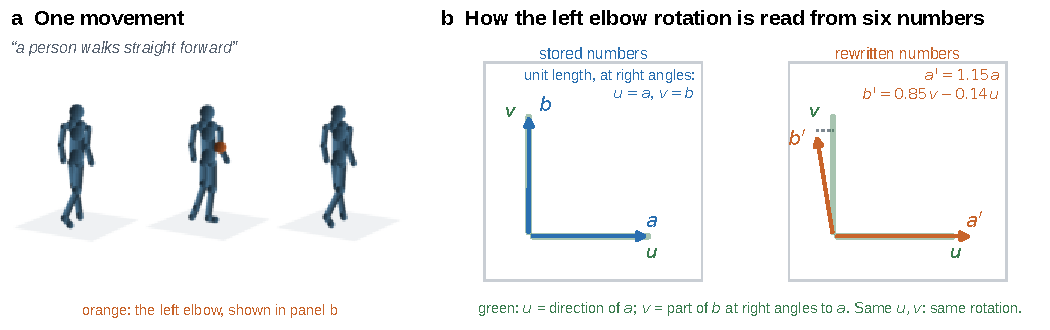
\includegraphics[width=\textwidth]{figures/teaser.pdf}
\captionof{figure}{\textbf{The movement stays fixed; the reported score changes.} Original and recoded features produce identical joint positions and represented rotations. The illustration renders the first fixed MDM example with the same procedural geometry and camera. Scores summarize a caption-targeted attack on 1,024 outputs, rather than this one clip. Canonicalization maps the two rotation encodings to the same representative.}\label{fig:teaser}
\end{@twocolumnfalse}}]

\begin{abstract}
Motion metrics should depend on represented movement, not on redundant coordinates of its encoding. We isolate a violation of this requirement in learned evaluators of continuous rotation features. Positive rescalings and shear preserve every joint rotation while positions, velocities, contacts and timing remain fixed. A fixed, caption-independent recoding changes HumanML3D FID by up to 3.57 at zero physical displacement. Public-output audits reveal smaller signed differences across HumanML3D and KIT-ML, whose direction varies by release and reader. Caption-targeted retrieval rises from 0.397 to 0.993; a distinct Transformer evaluator is also susceptible. Caption-blind attacks transfer between checkpoints of the same architecture. Without an attack, canonicalizing real How2Sign inputs changes 1,438 of 2,183 decoded sentences despite nearly unchanged BLEU. Source-conditioned layers also redirect backtranslation in three sign-language corpora. Unlike essential-feature evaluation, converter-based canonicalization retains every represented rotation, making it applicable to rotation-only domains. We provide controlled audits and a portable evaluation contract that make scores invariant to equivalent rotation encodings without claiming improved motion or universal evaluator accuracy.
\end{abstract}

\section{Introduction}
Motion generation is compared through learned retrieval and distribution metrics. These scores should remain unchanged when the movement being evaluated remains unchanged. Yet a fixed rescaling and shear of rotation features can create a large FID difference between two copies of the same HumanML3D motion. With evaluator gradients, the same operation can push retrieval toward a chosen caption while leaving the generated movement untouched (\cref{fig:teaser}). The evaluator is responding to the representation as well as the movement.

This matters before considering an adversary. Learned text--motion embeddings underpin widely used scores for public generators~\cite{guo2022,tevet2023,mld2023,t2mgpt2023,motionlcm2024}. A representation-dependent score combines two effects: differences in the generated motion and differences in how that motion is encoded. These metrics are already imperfect proxies for human judgment~\cite{stein2023}; invariance to physically equivalent encodings is a separate, testable requirement. It can be checked without assuming that a metric perfectly captures human preferences.

The source of the failure is simple. Continuous 6D rotation features~\cite{zhou2019} use two vectors whose normalization and orthogonalization determine a rotation. Positive scales and shear alter the vectors without altering that rotation. A renderer or forward-kinematics converter discards these redundant coordinates. A learned evaluator receiving the raw vectors need not discard them. We use this known equivalence to change only the rotation encoding, holding positions, root trajectory, velocities, contacts and timing fixed. Native geometry checks verify that the score changes occur at identical represented movement.

Meng et al.~\cite{mardm2025} identify redundancy-related evaluation bias and train HumanML3D readers on root motion and local positions. Their block-noise tests also change represented rotations and other features. Our question is more specific: \emph{can equivalent encodings of the same rotations receive different scores?} We isolate the converter's exact equivalence class, with equal-budget block controls and paired public-output audits.

The distinction determines which remedy is available. HumanML3D includes a position channel, so an essential-feature reader can discard rotations. The sign-language representations studied here contain only body and hand rotations: discarding that block discards their entire movement input. Even without an attack, canonicalizing real sign inputs changes many decoded sentences while aggregate BLEU barely moves. Canonicalization retains every represented rotation, testing a requirement that position-only evaluation cannot satisfy.

We build the evidence in increasing order of access. Fixed recodings use neither captions nor evaluator gradients. Paired audits test unmodified public outputs, where the effects are smaller and change sign. Target-aware attacks measure channel capacity in two evaluator architectures. Caption-blind attacks use only TRAIN motion statistics and transfer to another checkpoint without its gradients. Finally, TRAIN-fitted layers redirect sign-language backtranslation on generated and real motion. These experiments address one question throughout: whether a reported score is determined by the movement or by its encoding.

Canonicalization provides a direct remedy. Applying the evaluator's rotation converter before normalization gives every equivalent encoding the same representative. This closes the rotation channel without removing rotational information. We distinguish this invariance guarantee from accuracy and specify the converter, normalization and masking rules needed to implement it.

Our contributions are:
\begin{itemize}
\item An exact-equivalence audit that isolates rotation-encoding dependence, with equal-budget controls and paired public-output tests on HumanML3D and KIT-ML.
\item A demonstration of score manipulation at unchanged movement across two motion-evaluator architectures and three sign-language corpora, including caption-blind checkpoint transfer.
\item A canonicalization contract that retains all rotations, including in rotation-only domains, supported by native geometry checks and physical-noise calibration.
\end{itemize}

\section{Related work}
\paragraph{Motion representation and evaluation.}
Continuous rotation representations~\cite{zhou2019} and rotation projections~\cite{levinson2020} establish the geometric operations used here. HumanML3D's learned evaluator~\cite{guo2022} consumes positions, velocities and rotation features; TMR~\cite{tmr2023} learns retrieval with a Transformer. We audit public outputs from diffusion, consistency and token-based releases~\cite{tevet2023,mld2023,motionlcm2024,t2mgpt2023,momask2024,motiondiffuse2024,closd2025}. MARDM~\cite{mardm2025} perturbs redundant rotation, velocity and contact blocks and retrains GRU/CLIP readers using its 67 essential features. Those interventions need not preserve represented rotations. We isolate exact rotation equivalence and retain rotational information, including in domains lacking a separate position channel. Our audit addresses within-rotation encoding dependence rather than the whole redundancy mechanism or a new rotation representation.

\paragraph{Adversarial evaluation.}
Universal perturbations and perturbation-generating networks demonstrate that neural predictions can be redirected~\cite{uap2017,gap2018,atn2018}. Related attacks target recognition, translation, learned image quality and motion prompts~\cite{li2023,liu2024,huang2023,alertmotion2025,fang2025}. Our constraint is stronger than a small numerical perturbation: decoded rotations and every nonrotation motion channel are preserved. Detector-aware controls~\cite{tramer2020adaptive} and physical perturbations help separate this representation channel from broader adversarial robustness. Reward fine-tuning motivates the distinction between a controllable evaluator and exploitation during generator training~\cite{draft2024,tan2026,motionrft2026,solireward2026}.

\paragraph{Sign-language backtranslation.}
Production on PHOENIX-2014T, How2Sign and CSL-Daily~\cite{camgoz2018,duarte2021,zhou2021} is evaluated with motion-to-text readers~\cite{saunders2020,camgoz2020,walsh2025,signsparkbt}. SiLVERScore and BackTranslation 2.0 study richer semantic and prosodic evaluation~\cite{imai2025,cory2026}. We examine a representation requirement complementary to linguistic assessment. A source-conditioned layer serves as an amortized attack; it does not improve the signing or replace human evaluation.

\section{An evaluation contract for rotations}
\subsection{The rotation equivalence class}
For a joint, let $d=(a,b)\in\R^6$ with $a\ne0$ and $b$ noncollinear with $a$. The Gram--Schmidt converter computes
\begin{align}
u&=a/\|a\|,\qquad b_\perp=b-(u^Tb)u,\nonumber\\
v&=b_\perp/\|b_\perp\|,\qquad R(d)=[u;v;u\times v].\label{eq:rotation}
\end{align}
Sign-language implementations use rows; HumanML3D/KIT use these vectors as columns. Each audit retains the native convention. For $\alpha,\beta>0$ and $\eta\in\R$, define
\begin{equation}
\G_{\alpha,\beta,\eta}(a,b)=(\alpha a,\beta b+\eta a).\label{eq:transform}
\end{equation}
The first normalized vector remains $u$; orthogonalizing the second gives $\beta b_\perp$. With $\C(d)=(u,v)$, exact arithmetic gives
\begin{equation}
R(\G(d))=R(d),\quad \C(\G(d))=\C(d).\label{eq:invariance}
\end{equation}
Conversely, every encoding of $(u,v)$ has $a=\rho u$, $b=\sigma v+\tau u$, with $\rho,\sigma>0$. Thus the transformation spans the nondegenerate rotation fiber. This follows from the established converter~\cite{zhou2019}; the contribution is to audit and close the channel it exposes to evaluation.



We apply $\G$ only to valid rotation blocks. Every other HumanML3D/KIT channel and padded frame is protected bitwise. For sign language, body/hand rotations, timing and other motion parameters remain fixed. Deterministic forward kinematics gives the same motion at fixed shape and translation. Native matrices, RIC positions and FK are checked independently of scores. Normalization clamps must remain inactive; finite-precision residuals and decoded hypothesis equality are verified separately.

\subsection{Auditing the channel at different access levels}
\paragraph{Fixed recodings and natural outputs.}
A fixed recoding uses $(\log\alpha,\log\beta,\eta)=(b,-b,b)$, independently of captions, with both signs and all tested magnitudes retained. Random recodings are another caption-independent control. Neither uses a trained attack or evaluator gradients. Natural-output audits instead compare each unmodified public output to its canonical representative.

\paragraph{Target-aware and caption-blind attacks.}
Per-clip attacks optimize coefficients with bounded parameterization
\begin{equation}
(\log\alpha,\log\beta,\eta)=b\tanh q.\label{eq:bounds}
\end{equation}
A caption-targeted attack minimizes frozen-reader loss toward an available caption. Circularly shifted captions test whether the reader follows an arbitrary target. Caption-blind attacks consume no caption content or TEST-reference embeddings: using source-evaluator gradients, regularized Gaussian transport~\cite{bhatia2017} maps generated motion embeddings toward statistics of TRAIN motion. Outputs are sealed before TEST-reference scoring. A different official checkpoint scores the sealed outputs without providing attack gradients or target statistics.

\paragraph{Learned sign-language layers.}
A layer $h_\theta(x,c)$ predicts the same bounded coefficients from motion $x$ and source caption $c$. Only the layer is fitted on TRAIN caption loss; generator and reader remain frozen. Final backtranslation receives features, lengths and masks. Source text is available to the layer, making this an amortized, target-aware attack. Motion-only and canonical-loss controls isolate the role of that source information.

\subsection{Closing the channel}
For a deterministic reader $f$, canonicalization satisfies
\begin{equation}
(f\circ\C)(\G(x))=(f\circ\C)(x).\label{eq:closure}
\end{equation}
The guarantee holds for every admissible scale and shear, independently of the attack target. It retains all represented rotations and closes the channel before the reader can use it. A detector, by contrast, must recognize an unfamiliar encoding. In the supplement, an adaptive attack preserves both canonical distance and squared 6D norm yet changes backtranslation, demonstrating the limitation of those detector statistics.

The portable implementation applies $\C$ to unnormalized features, preserves padding and nonrotation channels, and rejects zero or collinear vectors on valid frames. Its evaluation contract specifies converter convention, normalization, masking and consistent reader fitting/inference. Invariance does not imply accuracy. Already canonical real-motion features provide an implementation sanity check; noncanonical sign-language data allow a separate matched reader-adaptation comparison.

Normalization order matters. With feature normalization $\mathcal N$ and frame mask $m$, the defended interface is $f(\mathcal N(\C(x)),m)$. Projecting already standardized vectors generally does not implement the native rotation converter. Our paired audits keep evaluator weights, normalization statistics and reference embeddings fixed. A canonical evaluation protocol should apply the defended interface to both evaluated and reference motion; a newly fitted reader can learn on canonical inputs throughout. This makes the handling of equivalent encodings part of the evaluation interface, rather than a detector threshold. \Cref{fig:portable} gives a guarded input interface.

\section{Experimental setup}
\paragraph{Motion datasets and evaluators.}
HumanML3D has 263 features, with 21 rotations in channels 67--192. Native KIT-ML~\cite{kit2016} has 251 features, with 20 rotations in 64--183. The Guo evaluator excludes only the four contact channels. Two official checkpoints share a Conv/BiGRU architecture with different weights. TMR uses an ACTOR Transformer, DistilBERT, its own normalization, deterministic VAE mean and cosine similarity. Its architecture differs from Guo's; our compatible-cohort audit does not reproduce TMR's full official annotation/filtering protocol. We use the native 251-feature KIT evaluator, not TMR's incompatible 263-feature KIT-AMASS model.

\paragraph{Paired public-output audit.}
Each release has 20 native TEST draws, with paired outputs, captions, candidate groups and reference. HumanML reference draws contain all 4,640 eligible segmented/mirrored entries after dropping an incomplete batch. MDM/MotionDiffuse/DiP emit 1,024 outputs; the other releases emit 4,640. KIT uses 704 outputs/reference. DiP receives 20 source prefix frames, excluded from the scored output, and is labeled as prefix-conditioned. These are consistency audits under recorded inference settings, not exact leaderboard reproductions. Paired $t_{19}$ intervals use separately specified comparison families; full FID/R1 results and published-error-bar context are in the supplement.

\paragraph{Controlled tests and physical checks.}
The targeted Guo study uses 1,024 fixed clips/source and five 32-candidate permutations. TMR uses the same 1,024 clips/source and native 32-candidate cosine retrieval. Both use 80 Adam steps and the final iterate. Fixed recodings retain both signs, smaller budgets and random controls. Angular calibration jointly updates rotations, FK positions, velocities and contacts, with fixed-per-clip and frame-independent axes. A common zero-angle reconstruction makes its comparisons coherent; its own score cost is reported. A generic TMR attack at matched numerical L2 is a supplemental physical-change control. Native geometry, saved metrics and canonical embeddings are independently verified.

\paragraph{Equal-budget block controls.}
All twenty saved real cohorts undergo rotation-fiber, outside-fiber rotation, velocity, contact and position interventions. We match $\|D_r^{-1}(y-x)\|_2=\kappa\sqrt L$ per clip, using reader $r$'s standard deviations $D_r$, valid length $L$ and radii $\kappa=1,3$. Each block has random controls and fixed directions with both signs. Non-null fixed directions use one local axis across joints and time; their scalars depend only on the input norm. Budgets include all 263 channels; Guo ignores contacts. Block-only controls can be physically inconsistent and differ from coherent angular calibration. Paired twenty-draw intervals adjust 28 original or 32 additional endpoints per reader, in separate families.

\paragraph{Rotation-only sign-language domain.}
Released 240-feature body/hand motion uses native filtering and backtranslation. Full TEST counts are 642 PHOENIX, 2,183 How2Sign and 1,162 CSL-Daily. BT readers share a Sign Language Transformer family~\cite{camgoz2020}; their real-motion BLEU is 15.00/3.48/6.89. Each learned layer uses three fitting seeds and final checkpoints. PHOENIX uses canonical generated motion; How2Sign/CSL use real motion. BLEU-4~\cite{papineni2002,post2018} is word-level on PHOENIX/How2Sign and character-level on CSL. Paired 20,000-sample intervals group How2Sign by 149 VIDEO\_IDs; seed-resampling sensitivity is separate~\cite{colas2018}. These public TEST splits were used during project development and are not project-wide untouched holdouts.

\section{Results}
\subsection{A fixed recoding changes FID without changing motion}
\begin{figure*}[t]\centering
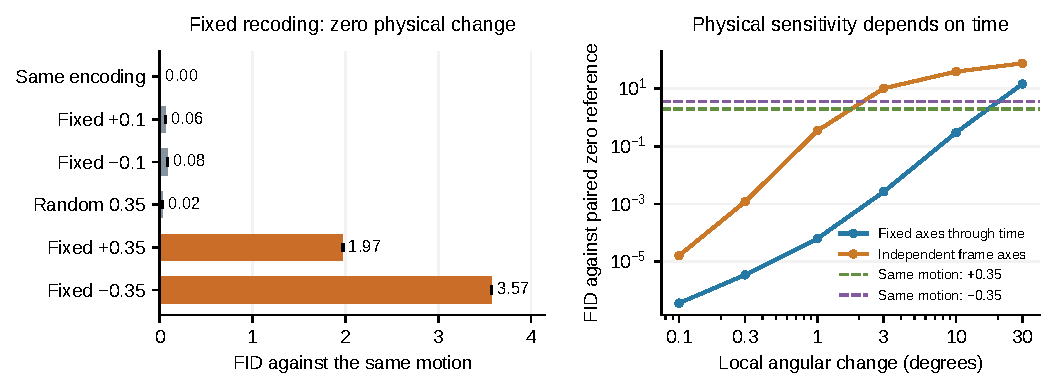
\includegraphics[width=\textwidth]{figures/encoding_and_physical_scale.pdf}
\caption{\textbf{A score difference needs no physical difference.} Left: fixed, caption-independent recodings of the same real HumanML3D motions; no optimization or gradients. Bars show means and 95\% $t_{19}$ intervals over 20 draws. Right: coherent angular perturbations on those motions, with two temporal noise structures. Both panels use the paired zero-angle reconstruction as reference; zero FID is by construction. Original-to-reconstruction FID is 0.0201. The recodings leave rotations and all nonrotation channels fixed.}\label{fig:encodingscale}\end{figure*}

\textbf{A deterministic recoding is sufficient to expose inconsistency.} On real HumanML3D motion, signed fixed coefficients $\pm0.35$ produce FID 1.97/3.57 against the same reconstructed motions (\cref{fig:encodingscale}). Positions and rotations are unchanged. This test uses no caption, no evaluator gradients and no fitted attack. Direction matters: fixed $\pm0.1$ and random coefficients produce much smaller changes. All these controls are shown together, rather than interpreting the largest recoding as a typical natural output.

\textbf{Physical calibration gives the score a measured scale.} The fixed-recoding FIDs lie between the measured 1- and 3-degree frame-independent perturbations, but between 10 and 30 degrees for temporally fixed axes. Updating all feature blocks requires coherent reconstruction, whose FID cost against the original data is 0.0201. Each comparison in the figure uses the same reconstructed motion and reference. The two curves show why there is no universal FID-to-degrees conversion; they contextualize evaluator sensitivity rather than human-perceived motion quality.

\begin{figure*}[t]\centering
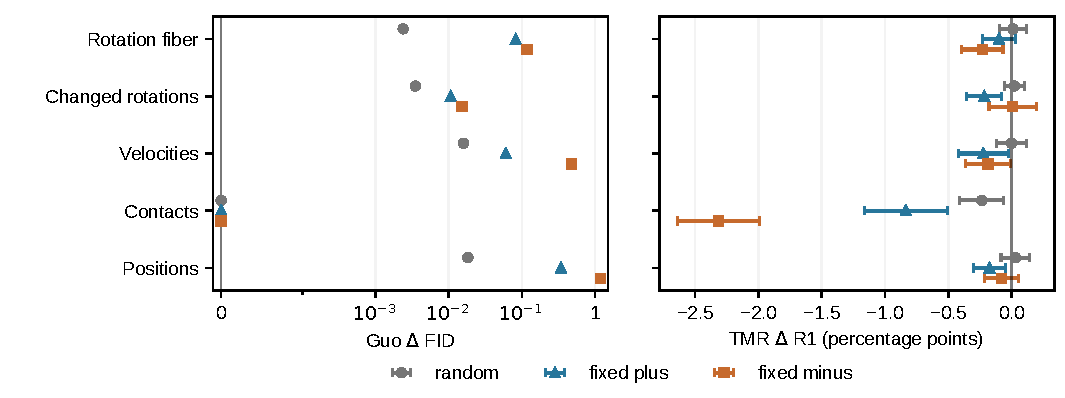
\includegraphics[width=\textwidth]{figures/matched_blocks.pdf}
\caption{\textbf{Direction controls qualify equal-budget block sensitivity.} Per-clip normalized L2 is $\kappa\sqrt L$, here $\kappa=3$, using each reader's own normalization. Random and both fixed signs are shown over twenty draws; original/additional intervals adjust 28/32 endpoints separately. Only the fiber interventions preserve rotations and every other block. Non-null directions are constant in time but can be inconsistent with fixed features. Guo excludes contacts. Both radii and all endpoints are supplemental.}\label{fig:matchedblocks}\end{figure*}

\textbf{Fixed directions can cause larger changes outside the fiber.} At $\kappa=3$, random velocity/position noise changes Guo FID by 0.016/0.018, exceeding random fiber coefficients (0.0024) and rotations (0.0035). Fixed position and fixed velocity directions reach 1.189 and 0.476, above the fixed fiber maximum of 0.117 (\cref{fig:matchedblocks}). Equal L2 alone does not establish a universal ranking of feature importance. The fiber's distinction is exact equivalence: only its interventions preserve rotations and every nonrotation feature.

\textbf{Sensitivity also depends on the reader.} Guo excludes contacts and its embeddings are unchanged by contact offsets. TMR reads them: at $\kappa=3$, a fixed negative contact offset reduces R1 by 2.32 percentage points, versus 0.23 for the fixed negative fiber direction. These are block-input controls, including nonbinary contacts, not motion-quality comparisons. Both signs, radii and all retrieval/cosine endpoints remain supplemental.

\subsection{The dependence also appears in public outputs}
\begin{table*}[t]
\centering\small\setlength{\tabcolsep}{5.5pt}
\caption{\textbf{Public outputs change FID at identical movement.} Twenty paired draws per release; $\Delta=\mathrm{raw}-\C$. Original five and additional HumanML/KIT studies each adjust ten FID/R1 endpoints separately. DiP uses a source prefix. Published FID and author margins give scale only: samples, readers and settings differ, precluding a cross-paper significance test. MDM50/DiP use corrected author results; T2M uses estimated length and MotionDiffuse its release preprint. Full sources/settings are supplemental.}\label{tab:editorialnatural}
\begin{tabular}{@{}lrrrrr@{}}\toprule
Release&Raw&$\C$&$\Delta$&95\% gap interval&Published FID\\\midrule
\multicolumn{6}{@{}l}{\emph{HumanML3D}}\\
MDM50&0.455&0.450&+0.0046&$[+0.00348,+0.00579]$&$0.489\pm.047$\\
MLD&0.445&0.449&-0.0038&$[-0.00519,-0.00237]$&$0.473\pm.013$\\
MotionLCM&0.575&0.606&-0.0315&$[-0.03473,-0.02822]$&$0.467\pm.012$\\
T2M-GPT&0.183&0.149&+0.0340&$[+0.03254,+0.03541]$&$0.141\pm.005$\\
T2M&1.393&1.347&+0.0464&$[+0.04414,+0.04858]$&$1.087\pm.021$\\
MoMask&0.068&0.064&+0.0033&$[+0.00279,+0.00382]$&$0.045\pm.002$\\
DiP (prefix)&0.367&0.365&+0.0015&$[+0.00004,+0.00303]$&$0.228\pm.027$\\
MotionDiffuse&0.977&0.981&-0.0041&$[-0.00737,-0.00076]$&$0.630\pm.001$\\
\midrule\multicolumn{6}{@{}l}{\emph{Native KIT-ML}}\\
MoMask&0.351&0.365&-0.0137&$[-0.02473,-0.00270]$&$0.204\pm.011$\\
MotionDiffuse&1.779&1.816&-0.0364&$[-0.04282,-0.03002]$&$1.954\pm.062$\\
\bottomrule\end{tabular}\end{table*}

\textbf{Unmodified releases are measurably representation-dependent.} Canonicalizing identical public outputs changes FID in all eight HumanML3D release settings and both native KIT settings (\cref{tab:editorialnatural}). Each reported FID interval excludes zero within its study's comparison family. In the original five-release audit, absolute gaps are at most 0.047; signs vary and the mean ranking is unchanged. This is inconsistency, not a finding of systematic inflation or intentional manipulation.

\textbf{Natural sensitivity depends on the reader.} Another official Guo checkpoint changes T2M's gap direction and makes MLD's FID gap inconclusive. TMR supplies a different architecture: its natural retrieval gaps are small, with positive intervals for MotionLCM and T2M and inconclusive intervals for the other audited releases. Thus the larger capacity demonstrated below should not be read as the prevalence of a large bias in existing generators. Full endpoints and intervals remain in the supplement.

\begin{figure}[t]\centering
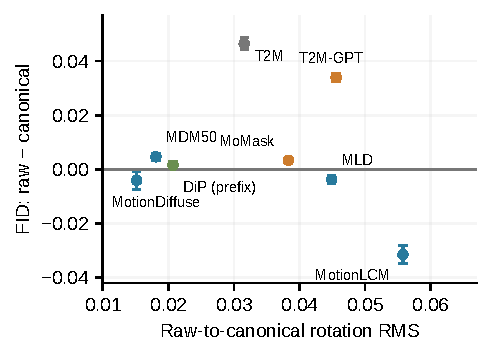
\includegraphics[width=\columnwidth]{figures/rotation_mechanism.pdf}
\caption{\textbf{Natural rotation deviations do not impose a uniform penalty.} Signed primary Guo FID gaps versus valid-frame raw-to-canonical rotation RMS for all eight release settings. Blue: diffusion/consistency; orange: VQ; gray: VAE; green: prefix-conditioned. Intervals are the original paired, family-adjusted gap intervals. Each point is one release's twenty-draw mean. Family and conditioning are confounded; this is a descriptive mechanism check.}\label{fig:rotationmechanism}\end{figure}

\textbf{Rotation noncanonicality alone does not explain a uniform diffusion penalty.} Three of four diffusion/consistency releases have negative raw-minus-canonical gaps, while both VQ releases have positive gaps (\cref{fig:rotationmechanism}); T2M's VAE has the largest positive gap overall. RMS correlates weakly with signed and absolute gaps across the eight releases, with no significant exact-permutation result. This counterfactual concerns only the rotation fiber. It neither tests velocity/contact errors nor refutes MARDM's full explanation of representation and diffusion-training effects.

\subsection{The channel can redirect two evaluator architectures}
\begin{table}[t]
\centering\footnotesize
\caption{\textbf{Two architectures can be redirected at fixed motion.} Caption-targeted R1 on the same 1,024 clips per source; frozen readers, 80 steps, bound 0.35. Each attack accesses its evaluator gradients and target caption. Native similarities and candidate permutations differ across architectures; compare within each row.}\label{tab:editorialretrieval}
\begin{tabular}{@{}llrrr@{}}\toprule
Reader&Motion&Clips&Original&Recoded\\\midrule
Guo&MDM&1,024&0.397&0.993\\
Guo&Real&1,024&0.462&0.996\\
\midrule
TMR&MDM&1,024&0.578&0.993\\
TMR&Real&1,024&0.688&1.000\\
\bottomrule\end{tabular}\end{table}

\textbf{Target-aware recoding can make retrieval nearly perfect at fixed motion.} Guo R1 rises from 0.397 to 0.993 on MDM and from 0.462 to 0.996 on real motion (\cref{tab:editorialretrieval}). TMR R1 rises from 0.578 to 0.993 on MDM and from 0.688 to 1.000 on real motion. Each attack has evaluator-gradient and caption access; native candidate permutations and similarity functions differ, so absolute scores should not be ranked across architectures. Native geometry remains fixed, while canonical embeddings change by at most $6.7\times10^{-6}$ in these targeted studies.

\textbf{The reader follows the target rather than a change in movement.} Shifted-caption attacks improve retrieval toward the shifted text while reducing agreement with the actual caption. Canonical-reader-gradient attacks fail to redirect retrieval. These controls isolate a manipulable representation channel. Retrieval improvement need not improve another metric: the targeted Guo attack worsens FID, as reported in the full endpoint table.

\subsection{Caption-blind manipulation transfers to another checkpoint}


\textbf{TRAIN motion statistics supply the attack targets.} Using only 2,048 TRAIN motion embeddings as targets, bound 0.1 reduces source-reader MDM FID by 39--53\% across three 960-output cohorts. The same protocol changes MLD FID from 0.706 to 0.289. It never consumes caption content or TEST-reference embeddings during optimization. Rotations and nonrotation channels remain unchanged.

\textbf{The effect survives a change in evaluator weights.} The sealed MLD attack changes FID from 0.659 to 0.579 in the destination checkpoint, which supplies no gradients or refitting. The MDM cohorts also improve there, with smaller gains than against the source reader (full curves are supplemental). The larger bound worsens every cohort in both checkpoints, showing that capacity does not imply a monotonic budget response. Canonical-gradient and random controls, and the cohort overlap counts, are reported in the supplement. This is checkpoint transfer within Guo's architecture, not transfer to TMR.

\subsection{Representation dependence in sign language}
\begin{table*}[t]
\centering\small
\caption{\textbf{Natural inputs, stability controls and learned layers.} Top: full test layer attacks, three fitting seeds, source text available; canonical hypotheses stay identical. Language tokenizations differ. Bottom: untargeted real-input changed percentages / NED, with Gaussian mean over three same-support fields and physical changes matched to the per-clip canonicalization norm. Paired intervals and one-degree controls are supplemental.}\label{tab:editorialsign}
\begin{tabular}{@{}llrrrrr@{}}\toprule
Corpus&Motion&Source raw&Layer raw&$\C$ before/after&Gain&95\% gain interval\\\midrule
PHOENIX&Generated&6.39&15.21&6.39&8.81&$[7.82,9.87]$\\
How2Sign&Real&3.48&6.11&3.48&2.64&$[2.27,3.03]$\\
CSL-Daily&Real&6.89&7.43&7.07&0.54&$[0.14,0.97]$\\
\midrule
\multicolumn{7}{@{}l@{}}{Real raw/$\C$ hypothesis changes: PHOENIX 0/642; How2Sign 1,438/2,183; CSL 464/1,162.}\\
\midrule
\multicolumn{7}{@{}l@{}}{Real-input controls: changed hypotheses (\%) / mean normalized edit distance}\\
Corpus&\multicolumn{2}{c}{Canonical}&\multicolumn{2}{c}{Gaussian matched}&\multicolumn{2}{c}{Physical matched}\\
How2Sign&\multicolumn{2}{c}{65.9 / 0.397}&\multicolumn{2}{c}{41.9 / 0.243}&\multicolumn{2}{c}{70.3 / 0.426}\\
CSL&\multicolumn{2}{c}{39.9 / 0.304}&\multicolumn{2}{c}{22.3 / 0.168}&\multicolumn{2}{c}{44.3 / 0.346}\\
\bottomrule\end{tabular}\end{table*}

\textbf{Real sign inputs show dependence without an attack.} Canonicalization changes 1,438/2,183 How2Sign and 464/1,162 CSL hypotheses, versus 0/642 on PHOENIX (\cref{tab:editorialsign}). BLEU changes only 3.4779 to 3.4840 and 6.8907 to 7.0662, respectively. These are paired decodes of real inputs under shared native preprocessing, with no layer, target caption or optimization; corpus BLEU can mask sentence-level changes.

\textbf{A TRAIN-fitted layer redirects backtranslation without changing signing.} On PHOENIX, the source-conditioned layer raises raw BLEU from 6.39 to 15.21, with unchanged canonical hypotheses (\cref{tab:editorialsign}). How2Sign and CSL-Daily extend the result to real motion: their gains are 2.64 and 0.54 BLEU. The layers use their corpus-specific encoders and receive source text; these are target-aware attacks, not improved signing or cross-language transfer.

\textbf{The effect depends on the representation channel.} Motion-only and canonical-loss ablations separate the role of source text from movement. Changing only the layer's text redirects the decoded caption while preserving physical rotations and canonical hypotheses. An adaptive per-clip attack further preserves canonical distance and squared 6D norm and still gains 4.09 BLEU on PHOENIX. Its full statistic-matching controls and failed learned variants remain in the supplement. Canonicalization closes the channel even when those scalar detectors do not detect it.

\subsection{Canonicalization closes the channel while retaining rotations}
\begin{table}[t]
\centering\footnotesize
\caption{\textbf{Essential-only evaluation is a different remedy.} Within-reader ranks of mean embedding FID over twenty common-reference draws. Guo $\C$ retains rotations; MARDM GRU/CLIP use 67 essential features. CLIP FID is descriptive. Ranks compare these saved release settings, not published leaderboards or evaluator accuracy.}\label{tab:mardmranks}
\begin{tabular}{@{}lrrr@{}}\toprule
Release&Guo $\C$&E-GRU&E-CLIP\\\midrule
MoMask&1&1&1\\
T2M-GPT&2&3&2\\
DiP (prefix)&3&2&3\\
MLD&4&4&4\\
MDM50&5&5&6\\
MotionLCM&6&6&5\\
MotionDiffuse&7&8&8\\
T2M&8&7&7\\
\bottomrule\end{tabular}\end{table}

\textbf{Discarding rotations and canonicalizing them are different remedies.} Public MARDM essential-only GRU/CLIP readers ignore rotation recodings exactly. With a common real reference across twenty draws, their mean-FID rankings differ from Guo $\C$ (\cref{tab:mardmranks}), both with Kendall agreement 0.857. Different features, weights and architectures contribute to these differences; they do not identify a better evaluator. In our rotation-only sign-language inputs, dropping rotations would remove all movement features. Canonicalization retains them and requires no replacement architecture.

\textbf{Equivalent encodings become equivalent evaluator inputs.} Applying $\C$ before normalization recovers the same canonical embeddings in the motion attacks and preserves every canonical decoded hypothesis in the sign-language attacks. The result follows from the converter contract, with native finite-precision checks verifying its implementation. A generic matched-L2 TMR attack that changes physical features remains effective after canonicalization; the defense targets equivalent encodings, not all adversarial perturbations.

\textbf{Accuracy requires a separate test on noncanonical inputs.} Real HumanML3D/KIT rotations are already canonical: their unchanged retrieval is an implementation sanity check, not evidence of a cost-free defense. For noncanonical sign-language features, matched raw/canonical reader adaptation gives How2Sign/CSL TEST differences of $+0.10/-0.02$ BLEU, with seed-plus-group intervals containing zero. This empirical comparison is distinct from the invariance guarantee; adaptation details are supplemental.



\section{Discussion}
Our results identify a concrete evaluation failure: the tested readers can distinguish encodings that their motion converters identify as the same movement. Fixed recodings establish this without a target or optimization. Public-output audits establish smaller natural dependence, with signs that vary by release and reader. Target-aware and caption-blind attacks demonstrate capacity under distinct access models. Canonicalization closes the rotation fiber while retaining rotational information.

\paragraph{Scope.}
This is an evaluation-consistency claim, not evidence of routine exploitation during generator training. The supplement reports unsuccessful reward-optimization pilots, released reward-trained checkpoints and ordinary-generator controls. TMR adds a distinct architecture under compatible cohorts rather than its full annotation protocol. BT readers share one family and have weak How2Sign/CSL accuracy; linguistic and human/avatar assessment is outside this study. Canonicalization closes the rotation-encoding channel, not positional/velocity redundancy or attacks that change movement.

\begin{figure}[t]
\centering\begin{minipage}{\columnwidth}\footnotesize
\begin{verbatim}
import numpy as np
from tools.canonicalize_motion import (
    canonicalize_motion,
)
def reader_input(raw, lengths, mu, sd):
    x = canonicalize_motion(raw, lengths)
    m = np.arange(x.shape[1])[None, :]
    m = m < lengths[:, None]
    z = (x - mu) / sd
    return z * m[..., None], m
\end{verbatim}
\end{minipage}
\caption{\textbf{A guarded HumanML3D/KIT input interface.} Use unnormalized motion and the reader's fixed normalization. The helper validates rotations and preserves protected channels. Apply the same masked interface to evaluated and reference motion.}\label{fig:portable}
\end{figure}

\FloatBarrier
\newpage
\section{Conclusion}
The same movement can receive different scores when a learned evaluator reads redundant rotation coordinates. We isolate this failure with transformations that preserve both positions and rotations, show that it occurs in public outputs, and demonstrate a larger controllable channel across motion retrieval and sign-language backtranslation. Canonicalization gives equivalent encodings a common input while retaining rotational information, while keeping accuracy a separate empirical question. Our evaluation contract and portable implementation make this requirement directly testable: a motion score should be specified on represented movement, with the treatment of equivalent encodings made explicit.

\clearpage
{\small\bibliographystyle{ieeenat_fullname}\bibliography{references}}
\end{document}
